% Chapter 3

\chapter{Heuristics on Word Length Similarity} % Chapter title

\label{ch:word} % For referencing the chapter elsewhere, use \autoref{ch:mathtest}

	\section{Guidelines for Feature Engineering in Ranking Functions}

The main idea of the information retrieval systems is to include a proximity score in conjunction to the ranking function. A proximity score is an application-dependent score, like page-rank metrics, contextual similarity and so on. The function should have well engineered feature embedded in itself and it should be able to generalize other results. The objectives of the ranking function are:

\begin{itemize}
	\item The score should be higher if the constituents of proximity score (real numbers or vectors) are similar.
	\item The proximity score should be below certain cut-off scores. These cut-off scores or limiting parameters can be determined through machine learning.
	\item The function should behave similar and able to generalize the behavior and working of the existing ranking functions in IR.
\end{itemize}

The assumption is taken that modeled function is bi-modal (as one has to consider extremities of the cut-off scores). Let $f(\mathbf{x}, \mathbf{y})$ be the modeled function, where $\mathbf{x}$ and $\mathbf{y}$ be the constituent vectors. In other words, this function determines similarity between $\mathbf{x}$ and $\mathbf{y}$ and it is a function of $d(\mathbf{x})$ and $d(\mathbf{y})$ where $d(\cdot)$ is the distance metric.


Length normalization functions, especially in the BM25 or pivoted length function are inversely proportional to the to the TF-IDF score. Thus, the model would be $f(\mathbf{x}, \mathbf{y})$ inversely proportional to the TF-IDF score.


\begin{equation*}
TF-IDF(q, d) \propto \frac{1}{f(\mathbf{x}, \mathbf{y})}
\end{equation*}

\subsection{Nature of the Function Curve}




Since the function has to be bi-modal distribution, distribution function would be modeled in the form asymmetrical inverted bell curve. Thus the trough of the curve should occur when distances of $\mathbf{x}$ and $\mathbf{y}$ are similar. In other words,

\begin{equation} \label{c1}
\frac{\partial f(\mathbf{x}, \mathbf{y})}{\partial ( d(\mathbf{x}) )} = 0 \text{ if } d(\mathbf{x}) \approx d(\mathbf{y})
\end{equation}

Similarly it can be shown that,

\begin{equation*}
\frac{\partial f(\mathbf{x}, \mathbf{y})}{\partial (d(\mathbf{y}))} = 0 \text{ if } d(\mathbf{x}) \approx d(\mathbf{y})
\end{equation*}

From here onwards, arguments would be taken from the $d(\mathbf{x})$ perspective, as $d(\mathbf{y})$ would have similar arguments.

The function should decrease monotonically if $d(\mathbf{x}) < d(\mathbf{y})$. In other words, 

\begin{equation} \label{c2}
\frac{\partial f(\mathbf{x}, \mathbf{y})}{\partial ( d(\mathbf{x}) )} < 0 \text{ if } d(\mathbf{x}) < d(\mathbf{y})
\end{equation}

The function should increase monotonically if $d(\mathbf{x}) > d(\mathbf{y})$. In other words,

\begin{equation} \label{c3}
\frac{\partial f(\mathbf{x}, \mathbf{y})}{\partial ( d(\mathbf{x}) )} > 0 \text{ if } d(\mathbf{x}) > d(\mathbf{y})
\end{equation}

\subsection{Nature of the Limits of the Curve}

Here the left extremity of the curve could be bounded to the parameter $b_1$.
\begin{equation} \label{c4}
\lim_{d(\mathbf{x})\to 0} f(\mathbf{x}, \mathbf{y}) = b_1
\end{equation}

Similarly, the right extremity of the curve could be bounded to the parameter $b_2$.
\begin{equation} \label{c5}
\lim_{d(\mathbf{x})\to \infty} f(\mathbf{x}, \mathbf{y}) = b_2
\end{equation}

The trough of the curve exists when $\frac{\partial f(\mathbf{x}, \mathbf{y})}{\partial ( d(\mathbf{x}) )} = 0$. Thus the limit is set to 1. It can not be set it to 0, because $f(\mathbf{x}, \mathbf{y})$ lies in the denominator of the scoring function.
\begin{equation} \label{c6}
\lim_{d(\mathbf{x})\to d(\mathbf{y})} f(\mathbf{x}, \mathbf{y}) = 1
\end{equation}

The specific case of these guidelines can be applied to the recommendation systems.

%----------------------------------------------------------------------------------------

\section{Design of the TAKE curve}

Here, the function would be modeled using Richard's curve. The curve is defined by,
\begin{equation}
g(x) = l + \frac{u - l}{(A + e^{{-B(x-M)}})^{{1/\nu }}}
\end{equation}

Here, $l$ is lower limit, $u$ is upper limit and $M, \nu, A, B$ are free parameters

The distance metrics are taken to be just real numbers. Thus, $d(\mathbf{x}) = x$ and $d(\mathbf{y}) = y$. The trough of the curve should occur when, $d(\mathbf{x}) = d(\mathbf{y})$ or $x = y$. The function can be partitioned into three parts:
\begin{itemize}
	\item monotonically decreasing Richard's curve, $g(x)$  when $x < y$
	\item monotonically increasing Richard's curve, $g(x)$ when $x > y$
	\item Value of heuristic function, $h(x, y) = 1$  when $x = y$
\end{itemize}

The definition of the function now looks like:

\begin{equation}
h(x, y) = 
\begin{cases}
g(x_1)       & \quad \text{if } x < y\\
1 & \quad \text{if } x = y\\
g(x_2)  & \quad \text{if } x > y\\
\end{cases}
\end{equation}

where $x_1 \in [0, y]$, $x_2 \in [y, \infty]$ and $x_1, x_2 \subset x$

Applying equation (\ref{c1}), the constraint obtained is:

\begin{equation}
\frac{\partial h(x, y)}{\partial x}\at[\bigg]{x=y} = 0
\end{equation}

From equation (\ref{c2}), the constraint obtained is:

\begin{equation*}
\frac{\partial g(x_1)}{\partial x_1} < 0
\end{equation*}

From equation (\ref{c3}), the constraint obtained is:

\begin{equation*}
\frac{\partial g(x_2)}{\partial x_2} > 0
\end{equation*}


From limiting condition (\ref{c4}), the constraint obtained is: 

\begin{align}
\lim_{x_1 \to 0} g(x_1) &= b_1 \\
\frac{\partial g(x_1)}{\partial x_1}\at[\bigg]{x_1 = 0} &\approx 0
\end{align}

From the limiting condition (\ref{c5}), the constraint obtained is: 

\begin{align}
\lim_{x_2 \to \infty} g(x_2) &= b_2 \\
\frac{\partial g(x_2)}{\partial x_2}\at[\bigg]{x_2 = \infty} &\approx 0
\end{align}

From the limiting condition (\ref{c6}), the constraint obtained are: 

\begin{align}
\frac{\partial g(x_1)}{\partial x_1}\at[\bigg]{x_1 = y} &\approx \frac{\partial g(x_2)}{\partial x_2}\at[\bigg]{x_2 = y} &\approx 0  \\
\lim_{x_1 \to y} g(x_1) &= \lim_{x_2 \to y} g(x_2) &= 1 
\end{align}

After solving the constraints, and using the binomial approximation for small $\nu$, the solutions obtained are:

\begin{equation}
h(x, y) = 
\begin{cases}
1 + \frac{b_1 - 1}{1 + e^{B_1(x - cy)}}       & \quad \text{if } x < y\\
1 & \quad \text{if } x = y\\
1 + \frac{b_2 - 1}{1 + e^{-B_2(x - (1 + c)y)}}  & \quad \text{if } x > y\\
\end{cases}
\end{equation}

where,

\begin{itemize}
	\item $B_1$ and $B_2$ are growth parameters, can be typically set to 1
	\item $c$ is the trough curvature, where $c \in (0, 1)$
\end{itemize}

According to the requirements, length similarity would be rewarded between query and document lengths. In that case, $x = |d|$ and $y = |q|$. Intuitively, that means the value of the scoring function will be higher if $|d| \approx |y|$.

Substituting the values, we get:

\begin{equation}
h(|d|, |q|) = 
\begin{cases}
1 + \frac{b_1 - 1}{1 + e^{B_1(|d| - c|q|)}}       & \text{if } |d| < |q|\\
1 &  \text{if } |d| = |q|\\
1 + \frac{b_2 - 1}{1 + e^{-B_2(|d| - (1 + c)|q|)}}  &  \text{if } |d| > |q|\\
\end{cases}
\end{equation}

This feature can now be substituted in the ranking function in place of length normalization function. For example, the original BM25 function is:

\begin{align*}
score(q, d) = & \sum_{t \in d \cap q} f(t, q) \log \frac{M + 1}{df(t)} \times \\
& \frac{ (k + 1) f (t, d) }{f(t, d) + k \left( 1 - b + b \frac{|d|}{avgdl} \right)} 
\end{align*}

The normalization feature $\left( 1 - b + b \frac{|d|}{avgdl} \right)$ in the BM25 formula can be replaced with $h(|d|, |q|)$ to get our desired ranking function:
\begin{equation}
\label{heuris}
\begin{aligned}
score(q, d) = & \sum_{t \in d \cap q} f(t, q) \log \frac{M + 1}{df(t)} \times \\
& \frac{ (k + 1) f (t, d) }{f(t, d) + k \left( h(|d|, |q|) \right)}  \\
\end{aligned}
\end{equation}

\section{Description of TAKE}

The lengths of the misspelled word and correctly spelled word should almost be similar. 
Usually edit distance between misspelled and correctly spelled word are around 1 or 2.
The idea here is to reward the documents more in which document length and query length are closer to each other, and similarly penalize the extremely dissimilar lengths.

Let $|q|$ be the query length and $|d|$ be the document length. Let $h(|q|, |d|)$ be the heuristic function to calculate length similarity. 

The objective of the heuristic function should be:
\begin{enumerate}
	\item $h(|q|, |d|)$ should increase if $|q|$ and $|d|$ are dissimilar
	\item Similarly, $h(|q|, |d|)$ should decrease if $|q|$ and $|d|$ are similar
\end{enumerate}

Here we have used two variants.

\section{Power penalization} This uses hyperparameter $\gamma$ which varies from $[0, 1]$.
\begin{equation}
	\begin{aligned}
		h(|q|, |d|) = (||q| - |d|| + 1)^\gamma
	\end{aligned}
\end{equation}

The nature of the curve is plotted in Figure \ref{natures}.
\begin{figure}[h]
	\centering
	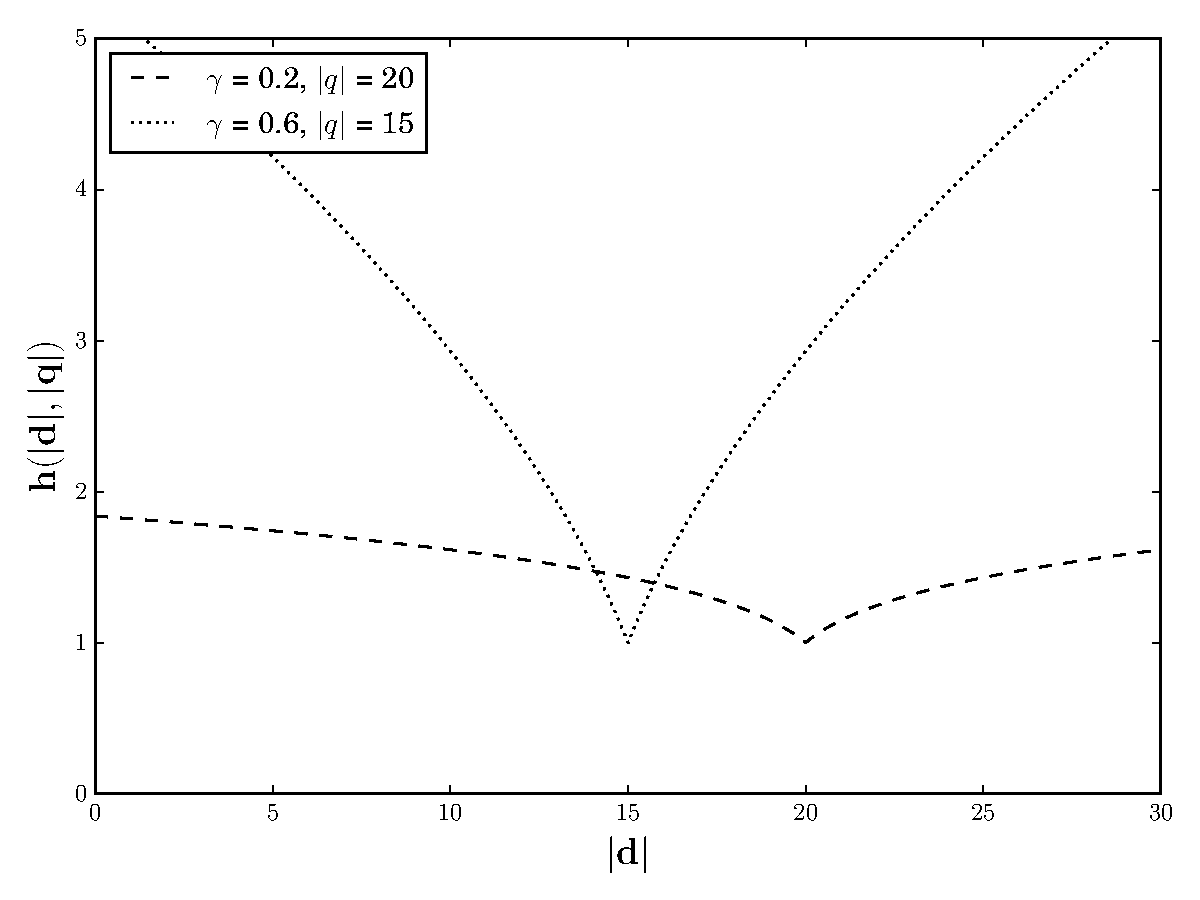
\includegraphics[width=\textwidth]{gfx/test1.pdf}
	\caption{The nature of power penalization $h(|d|, |q|)$ curve. The value of $h(|d|, |q|)$ dips when $|d|$ approaches the $|q|$. As the $\gamma$ increases, penalization would become more harsher.}
	\label{natures}
\end{figure}

\section{Bucket-shaped sigmoidal penalization} 

Here, the function would be modeled using Richard's curve, also known as generalized sigmoidal curve \cite{birch1999new}. 
The curve is defined by,
\begin{equation}
	g(x) = l + \frac{u - l}{(A + e^{{-B(x-M)}})^{{1/\nu }}}
\end{equation}

Here, $l$ is lower limit, $u$ is upper limit and $M, \nu, A, B$ are free parameters

As compared to normal sigmoid function, this function allows more flexibility in the choice of the parameters.
Since, we have to model a penalization function, the aim would be to model a "trough" in the curve as $|q|$ approaches towards $|d|$. 
We divide this function into three parts:

\begin{itemize}
	\item monotonically decreasing Richard's curve, $g(x_1)$  when $|d| < |q|$, or $\frac{\partial g(x_1)}{\partial x_1} < 0$
	\item monotonically increasing Richard's curve, $g(x_2)$ when $|d| > |q|$, or $\frac{\partial g(x_2)}{\partial x_2} > 0$
	\item Value of heuristic function, $h(|d|, |q|) = 1$  when $|d| = |q|$
\end{itemize}

where $x_1 \in [0, |d|]$, $x_2 \in [|d|, \infty]$ and $x_1, x_2 \subset |q|$. If we solve the limiting derivatives, use binomial approximations and remodel our parameters, we get the following penalization function:

\begin{equation}
	h(|d|, |q|) = 
	\begin{cases}
		1 + \frac{b_1 - 1}{1 + e^{B_1(|d| - c|q|)}}       & \text{if } |d| < |q|\\
		1 &  \text{if } |d| = |q|\\
		1 + \frac{b_2 - 1}{1 + e^{-B_2(|d| - (1 + c)|q|)}}  &  \text{if } |d| > |q|\\
	\end{cases}
\end{equation}

where, 

\begin{itemize}
	\item $b_1$ is the upper limit on the left side
	\item $b_2$ is the upper limit on the right side
	\item $B_1$ and $B_2$ are growth parameters, can be typically set to 1
	\item $c$ is the trough curvature, where $c \in (0, 1)$
\end{itemize}

The nature of this feature can be plotted as shown against various parameters (Figure \ref{nature}).

\begin{figure}[h]
	\centering
	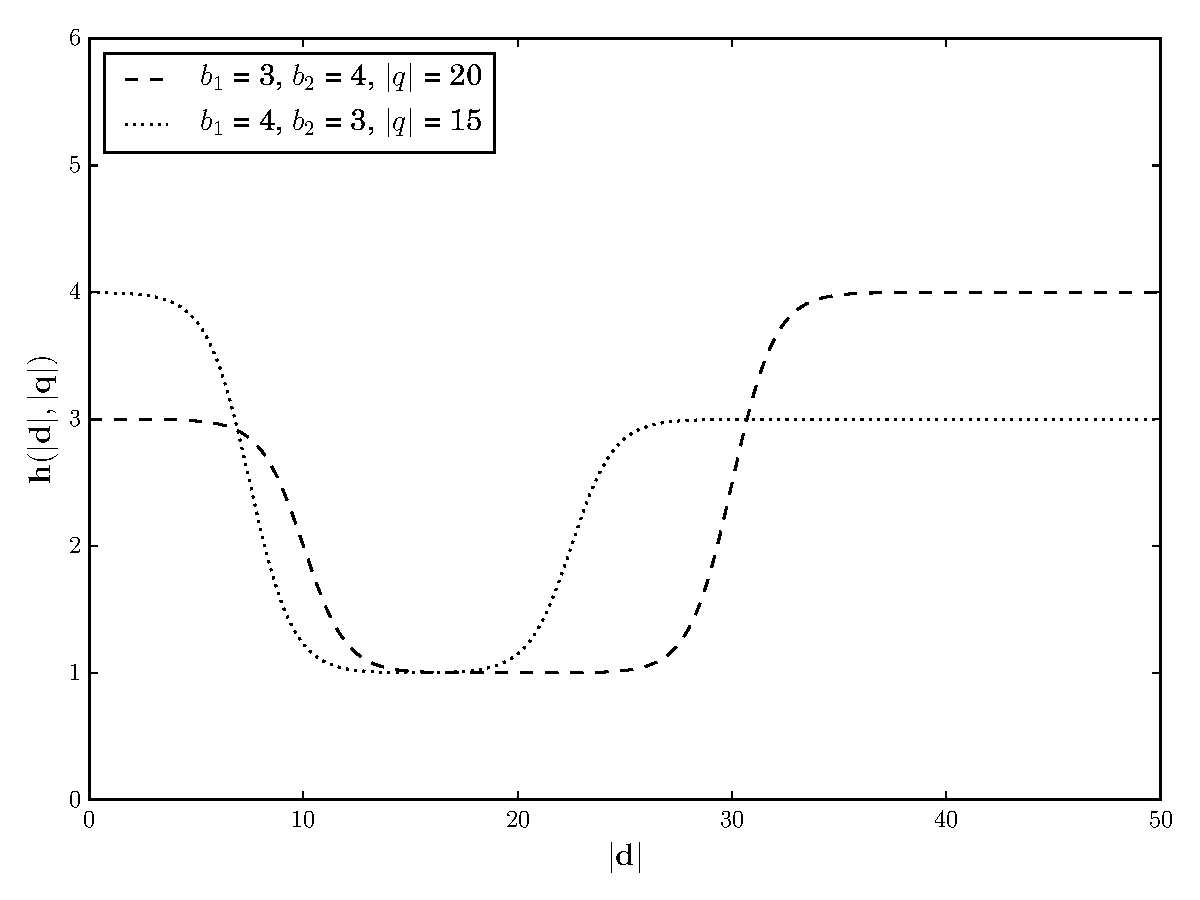
\includegraphics[width=\textwidth]{gfx/test.pdf}
	\caption{The nature of sigmoidal curve $h(|d|, |q|)$ with $B_1 = 1$, $B_2 = 1$ and $c = 0.5$}
	\label{nature}
\end{figure}

If we observe the graph we see a neat bucket-shaped trough when $|d|$ approaches $|q|$. It does not penalizes when the lengths are almost similar but starts penalizing when they are extremely dissimilar. This is feasible as a misspelling (query length) would be around the length of the correct spelling (document length). Using harsh penalization when lengths are dissimilar can prune unnecessary spelling matches with this heuristic.

Clearly, these two penalization heuristics could do behave and achieve the stated objectives. We now demonstrate how we can use this penalization heuristics in our ranking functions.

We know that BM25 ranking function is given by:

\begin{align*}
	score(q, d) = & \sum_{t \in d \cap q} f(t, q) \log \frac{M + 1}{df(t)} \times \\
	& \frac{ (k + 1) f (t, d) }{f(t, d) + k \left( 1 - b + b \frac{|d|}{avgdl} \right)} 
\end{align*}

where $f(t, q)$ is the frequency of terms in queries, $M$ is the number of documents, $k$ is a hyperparameter which sets the bound, $f(t, d)$ is the frequency of terms in documents, $df(t)$ is the document frequency, $b$ is the normalization parameter, $|d|$ is the document length and $avgdl$ is the average document length.

Here $\left( 1 - b + b \frac{|d|}{avgdl} \right)$ is the normalization heuristic. If we replace that heuristic with $h(|d|, |q|)$ we get:
\begin{equation}
	\label{heuris}
	\begin{aligned}
		score(q, d) = & \sum_{t \in d \cap q} f(t, q) \log \frac{M + 1}{df(t)} \times \\
		& \frac{ (k + 1) f (t, d) }{f(t, d) + k \left( h(|d|, |q|) \right)}  \\
	\end{aligned}
\end{equation}

If the value of $h(|d|, |q|)$ decreases, that is if $|d|$ and $|q|$ are similar, then the value of the $score(q, d)$ increases. This means similar document and query word lengths are rewarded. Vice versa can be said if the value of $h(|d|, |q|)$ increases.



We setup an experiment similar to section \ref{experim}, to analyze the behavior of these heuristics on the spelling dataset.
Here we vary $h(|d|, |q|)$ heuristic variants to evaluate their performances.
The results of the experiment are summarized in Table \ref{simexp}.

	Clearly, we see that sigmoidal penalty outperforms the other variants. 
However, sigmoidal penalization function is difficult to train due to large number of parameters.
Hence, we would only consider power penalization for the other experiments. 